\documentclass[a4paper,12pt]{article}

\usepackage{url}
\usepackage{epsfig}
\usepackage{graphics}
\usepackage{fancyhdr}
% \usepackage[backend=bibtex]{biblatex}

\graphicspath{{pictures/}}

\title{Word prediction performance of n-gram models applied to essentially different corpora}
\author{\hspace*{-0.5cm}
GROUP 34\\
\begin{tabular}{cccc}
Sofia Broom\'e & Jeremy Krebs & Valentin Geffrier & Erik Fredriksen \\
901210 & BIRTHDATE2 & BIRTHDATE3 & BIRTHDATE4 \\
sbroome@kth.se & MAIL2@kth.se & MAIL3@kth.se & MAIL4@kth.se \\
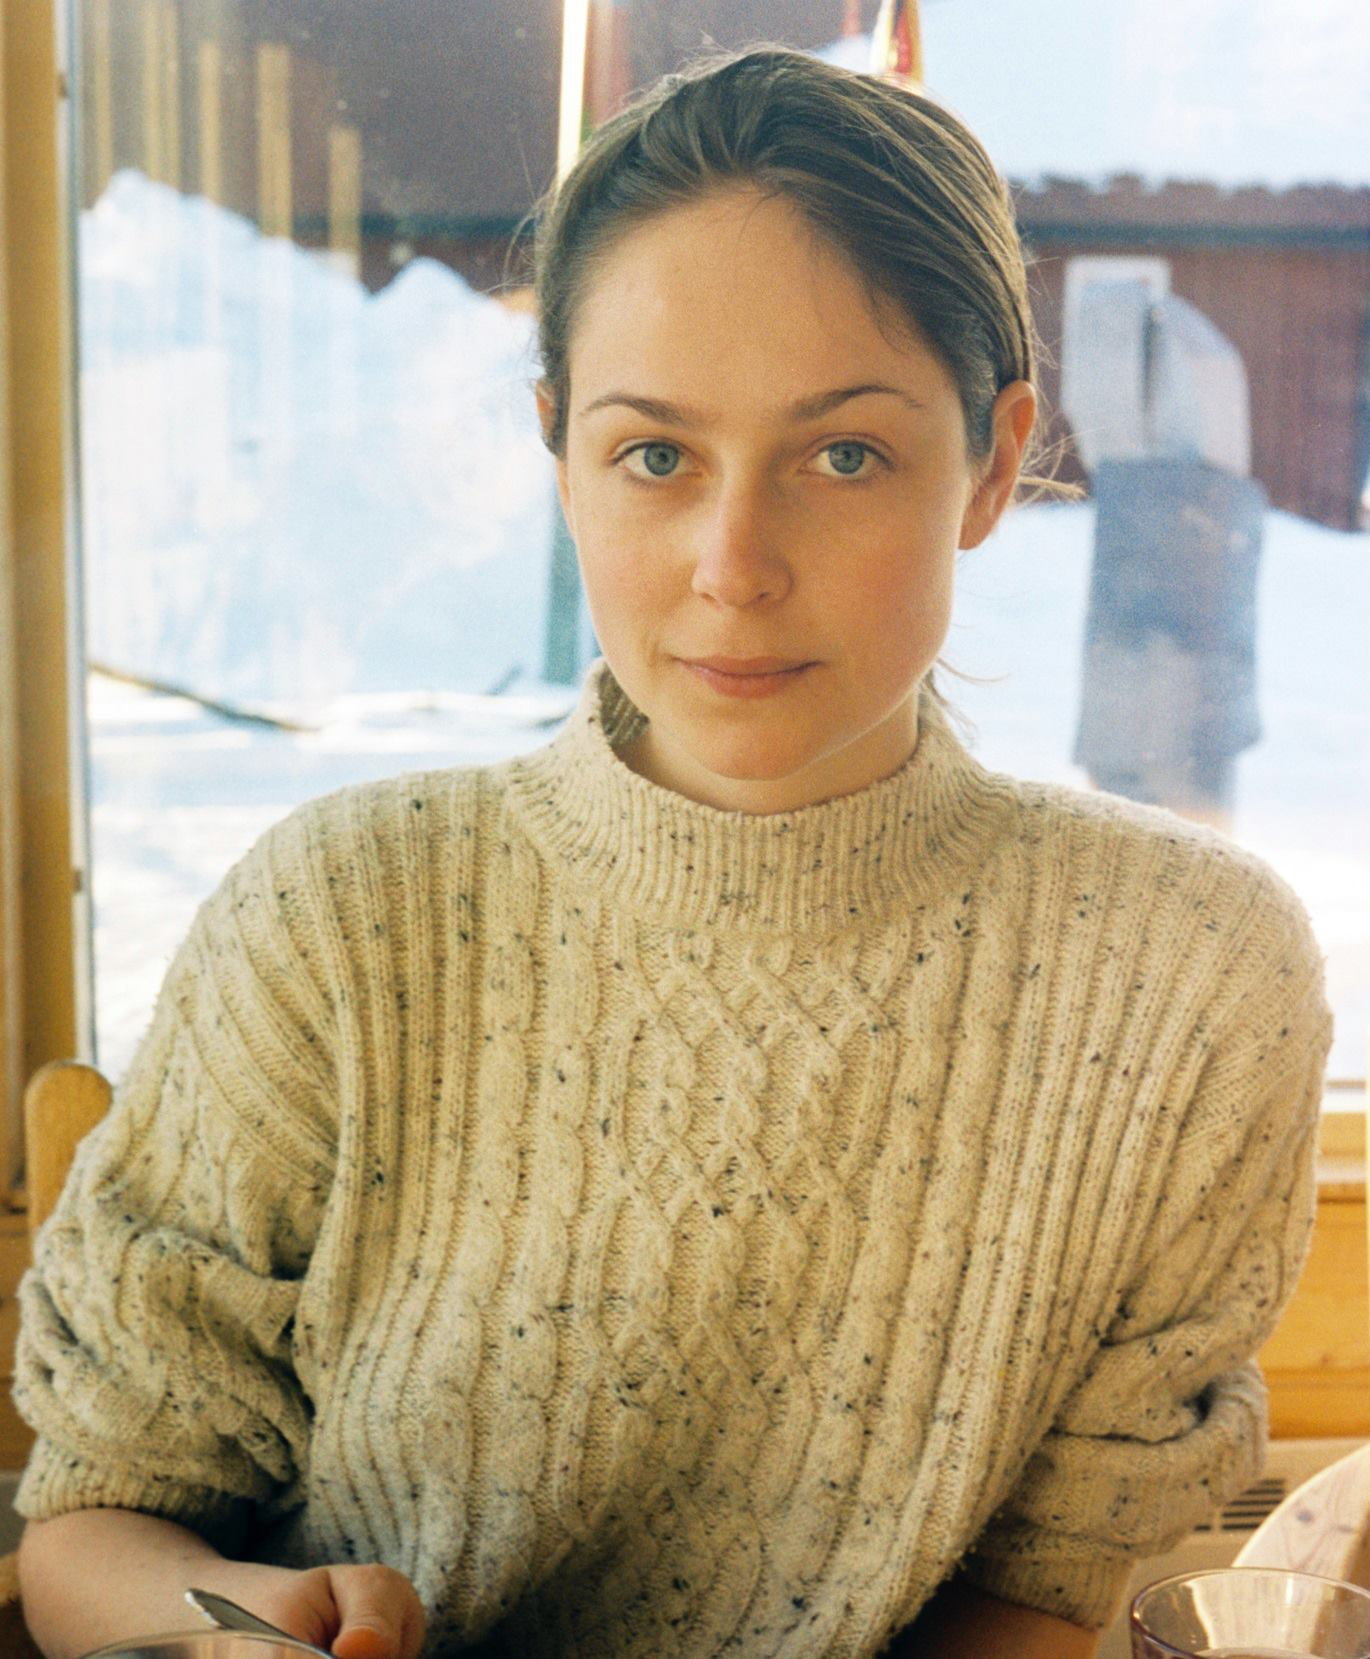
\includegraphics[width=0.13\linewidth]{Nikkaluokta} & 
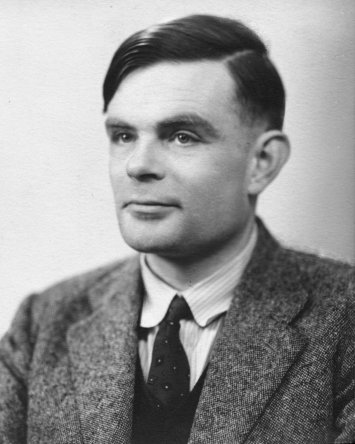
\includegraphics[width=0.13\linewidth]{Alan_Turing_photo} & 
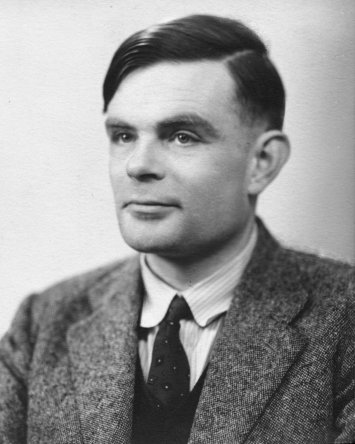
\includegraphics[width=0.13\linewidth]{Alan_Turing_photo} & 
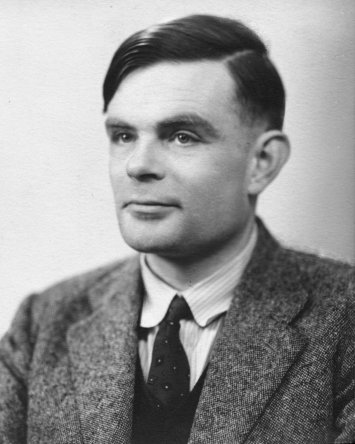
\includegraphics[width=0.13\linewidth]{Alan_Turing_photo}
\end{tabular}} 
% Normally there will not be any pictures but we want
% these so that we can connect faces to names in the course
% We also want birthdates so that we can tell people with the same
% name apart
\date{}

\pagestyle{fancy}
\setlength{\headheight}{15pt}
\fancyhf{}
\lhead{DD2380 ai15} % DO NOT REMOVE!!!!
\rhead{S. Broom\'e, J. Krebs, V. Geffrier, E. Fredriksen} %% UPDATE WITH YOUR NAMES

\begin{document}

\maketitle
\thispagestyle{fancy}

\begin{abstract}
Bla hej bla bla bla bla bla bla bla bla bla bla bla bla bla bla bla bla 
bla bla bla bla bla bla bla bla bla bla bla bla bla bla bla bla bla 
bla bla bla bla bla bla bla bla bla bla bla bla bla bla bla bla bla 
bla bla bla bla bla bla bla bla bla bla bla bla bla bla bla bla bla
\end{abstract}



\clearpage

%%%%%%%%%%%%%%%%%%%%%%%%%%%%%%%%%%%%%%%%%%%%%%%%%%%%%%%%%%%%%
%%%%%%%%%%%%%%%%%%%%%%%%%%%%%%%%%%%%%%%%%%%%%%%%%%%%%%%%%%%%%
\section*{NOTE}
\begin{itemize}

\item The following sections are arranged in the order they would appear in a scientific paper. We think that these sections need to be there and written. However, these are only guidelines and if you think that some of these sections or subsections are irrelevant to you, please feel free to remove them. Similarly, if you want to include more sections or subsections please go ahead. Also feel free to rearrange them according to your convenience, but keeping some common sense (eg.~Introduction cannot come after Conclusions).

\item \textit{Introduction, Related Works, Experimental Results, Discussions, Summary} are sections that MUST be contained.

\item In the section of your \textit{Method}: please do not list your project as log book entries, please talk about the final method you want to present to us. Talk about the method scientifically or technically and not as "I did this..." "Then I tried this..." "this happened...." etc.

\item Do not paste any code unless it is very relevant!

\item The section \textit{Contributions} is a place to express any difference in contributions. The default assumption is that you all agree that all of you had an equal part to play in the project.

\item We suggest that you try to write this as scientifically as possible and not simply like a project report. Good Luck!

\item Please remove \textbf{this} NOTE section in your final report.

\end{itemize}
\section{Introduction}
\label{sec:intro}

Being able to dissect, classify, analyze and reproduce language is a highly relevant task for various fields. In the realm of artificial intelligence, we want to give language to our agents by means of communicating with them. When we deal with natural language processing we say that we make language models. Seen as there is no finite set of rules that can describe, say, the entire English language in a complete sense, for pragmatic reasons our best option seems to be basing our models on probabilistic observations - regardless of Noam Chomsky's contempt\cite{JurafskyBook} for the notion of probability of a sentence.

At the foundation of every language model that wants to predict words is the concept of n-grams, a method based on probabilistic distributions over length n combinations of subsequent words. An n-gram is a Markov chain of degree n-1. This quite simple construct can capture many patterns in sentences. Even though it doesn't consider grammar explicitly, grammar will inevitably be built in. For instance, an adjective will in many cases be followed by a noun, or a pronoun by a verb, and thus a bigram composed of those two grammatical types in the mentioned order will score high in probability. 

An n-gram gives us context for words, albeit not the full one. Gao and Suzuki\cite{gao2004long} explore long distance dependency for words through word clusters and the linguistically motivated {\it function word skipping} method where function words such as "has", "a", "in", "and", "the", etc, are skipped in favor of more significant words, called head words. In our experiments however, we will not delve further into this subject.

N-grams can also be used in a meta-sense - for instance it's common for part-of-speech-taggers to use n-gram models where they tag the current word based on the last word's tag.

There are some practical issues with the classical n-gram model. What do we do with the n-grams that aren't in our training set and thus have zero probability assigned? This is where techniques of so called smoothing comes in so that our model doesn't fail on encountering a previously unseen word in the test set. In case we are dealing with a higher-order n-gram and we find it has no probability mass , we might want to "back off" from the higher order and estimate the probability for a conditioned unigram, meaning we temporarily look at a smaller portion of a word's history.

Furthermore, what kinds of test sets does our training set allow us to perform well on? One should train on a  corpus which is representative of the domain of the intended use. And what happens to our model when we apply it to languages with a higher degree of inflection like Swedish, Basque or German?

From the above examples we see that in many cases just using the n-gram model in itself will not suffice. Over the years, researchers in natural language processing have added a lot of tweaks to the original idea such as linear combinations of n-gams, cache language models, LSA-based language models and maximum entropy models, to name a few.

In what follows we will explore n-gram models of varying degrees on dito corpora and grammar to see which results are obtained under which circumstances.

\subsection{Contribution}
What should we write here?

\subsection{Outline}
Bla bla bla bla bla bla bla Section~\ref{sec:ngram} bla bla bla bla 
bla bla bla bla bla Section~\ref{sec:method} bla bla bla bla bla bla 
bla bla bla bla bla bla bla bla bla bla bla Section~\ref{sec:exps}
bla bla bla bla bla bla Section~\ref{sec:summary} bla bla bla bla bla

%%%%%%%%%%%%%%%%%%%%%%%%%%%%%%%%%%%%%%%%%%%%%%%%%%%%%%%%%%%%%
%%%%%%%%%%%%%%%%%%%%%%%%%%%%%%%%%%%%%%%%%%%%%%%%%%%%%%%%%%%%%
%%%%%%%%%%%%%%%%%%   NGRAM MODELS   %%%%%%%%%%%%%%%%%%%%%%%%%
%%%%%%%%%%%%%%%%%%%%%%%%%%%%%%%%%%%%%%%%%%%%%%%%%%%%%%%%%%%%%
%%%%%%%%%%%%%%%%%%%%%%%%%%%%%%%%%%%%%%%%%%%%%%%%%%%%%%%%%%%%%
\section{N-gram models}
\label{sec:ngram}

\subsection{Theory}
The first mathematical tool needed in all natural language processing experiment is n-gram models. Speech taggers, smoothing and other methods may not be implemented at first, but n-gram models are needed to predict the next likely words of a sentence.

These models are quite easy to understand: if n is a fixed integer, a n-gram model works as a Markov chain to predict the next word. A model is trained on a corpora C, for instance a book or a set of books, so that the probability of each n-gram in the language is learned by the model. The bigger the corpora the more accurate and reliable will be the model as it will have more data to compute probabilities of sequences. More precisely, the probability $p$ that the word $w_n$ follows the group of words $w_1 w_2 ... w_{n-1}$ is given by the following formula:

$$ p = p(w_n | w_1 .. w_{n-1}) = \frac{|{(w_1, .., w_{n-1}, w_n) \in C}|}{|{(w_1, .., w_{n-1}, x) \in C}|} $$

With this formula, it is possible to know the more likely next word of a sentence, but also to generate the end of the sentence, each new word selected at random using this probability distribution. Therefore, a n-gram which appeared a lot in a corpora is more likely to appear in the sentence generator. However, this also tells us that heuristically, we should expect different results from one corpora to another. For instance using corpora from Shakespeare, the generated sentences are likely to be more erratic than with a novel since Shakespeare's syntax and grammar are more complicated.

\subsection{Experiments}
\subsubsection{Parameter $n$}
	The first experiment we did was to try to understand the influence of n in our word predictor and how we could tune this parameter. In these experiments, only the corpora and n is changed - no parts of speech tagger or smoothing have been used. The figure \ref{carroll_tuning_n} shows multiple iterations of prediction of the end of the sentence "Alice was looking for" with n-gram models for n between 1 and 4. The corpora used was the novel "Alice in Wonderland" from Lewis Carroll, 1865. 
	
We should note that a 1-gram model is not a Markov model. It just predicts a word according to its frequency in a book, regardless of the previous words. As punctuation symbols are considered as words in this corpora, that explains why it predicts so many commas and apostrophes. 

A 2-gram model will only predict a word according to the immediately preceding word in the sequence. This explains why after words like "the" and "a" there are often adjectives or nouns. However, the prediction is still not perfect since 2-gram models seems a bit shallow.

With 3-gram models and 4-gram models one can see that the sentences are a bit more grammatically correct but there is still some issues since the English grammar and syntax are not used in these models. This is why this is necessary to implement taggers and use a model that takes into consideration the grammar and the syntax of a language. Another thing with 4-gram models is that we can see the predictions are quite close for different attempts. This is because the more words are fixed, the less freedom there is for the next word: there is less 2-gram starting with "for" than 4-grams starting with "was looking for" in the corpora.
	
If n is too low, the predictor works really bad because one or two words might not be enough to predict a likely next word. However if n is too big, the corpora need to be really big as well and contain enough different n-gram so that the predictor is more diversified.

\subsubsection{The corpora}
See \ref{tab:corpora1} for a table of our tested corpora.
\begin{table}
\begin{center}
\begin{tabular}{|c|c|c|}
\hline
Tested corpora & Year & Nr. of words \\ \hline
Moby Dick by Herman Melville & 1851 & 260819\\ \hline
Alice's Adventures in Wonderland by Lewis Carroll & 1865 & 34110 \\ \hline
The Bible & & 1010654 \\ \hline
Leaves of Grass by Walt Whitman & 1891 & 154883\\ \hline
Selected poems by William Blake & 1789 & 8354 \\ \hline
\end{tabular}
\caption{The corpora tested in the n-gram experiments.}
\label{tab:corpora1}
\end{center}
\end{table}


What is this? Saying something about our references?

%%%%%%%%%%%%%%%%%%%%%%%%%%%%%%%%%%%%%%%%%%%%%%%%%%%%%%%%%%%%%
%%%%%%%%%%%%%%%%%%%%%%%%%%%%%%%%%%%%%%%%%%%%%%%%%%%%%%%%%%%%%
\section{Method}
\label{sec:method}

Starting from the Natural Language Toolkit (NLTK), we experimented with the different methods provided there. After a while we realized that this collection had some broken classes, notably the n-gram class with smoothing methods, which was essential to our experimenting. We thus resorted to the smoothing methods hopefully provided by spaCy, according to our project plan, but well there stumbled upon more problems, in that they provide no explicit methods for creating n-grams or smoothing. This took us outside the scope of the project plan, towards SRILM, a powerful tool for building statistical language models.

For the word prediction without smoothing we however stuck to NLTK but with our own implementations of n-gram-models. We made an abstract n-gram model class from which a bigram-, trigram-, and n-gram-class inherited.

\subsection{Implementation}
\label{sec:impl}

Erik writes something about his implementation of SRILM. Doesn't have to be long but just so we have something on smoothing.

Something about our thoughts behind the abstract class + ngramclasses...

%%%%%%%%%%%%%%%%%%%%%%%%%%%%%%%%%%%%%%%%%%%%%%%%%%%%%%%%%%%%%
%%%%%%%%%%%%%%%%%%%%%%%%%%%%%%%%%%%%%%%%%%%%%%%%%%%%%%%%%%%%%
\section{Experimental results}
\label{sec:exps}

Bla bla bla bla bla bla bla bla bla bla bla bla bla bla bla bla bla 
bla bla bla bla bla bla bla bla bla bla bla bla bla bla bla bla bla 
bla bla bla bla bla bla bla bla bla bla bla bla bla bla bla bla bla 

\subsection{Experiemntal setup}
Bla bla bla bla bla bla bla bla bla bla bla bla bla bla bla bla bla 
bla bla bla bla bla bla bla bla bla bla bla bla bla bla bla bla bla 
bla bla bla bla bla bla bla bla bla bla bla bla bla bla bla bla bla 

\subsection{Experiment ...}

Bla bla bla bla bla bla bla bla bla bla bla bla bla bla bla bla bla 
bla bla bla bla bla bla bla bla bla bla bla bla bla bla bla bla bla 
bla bla bla bla bla bla bla bla bla bla bla bla bla bla bla bla bla 

\begin{figure}
\centering
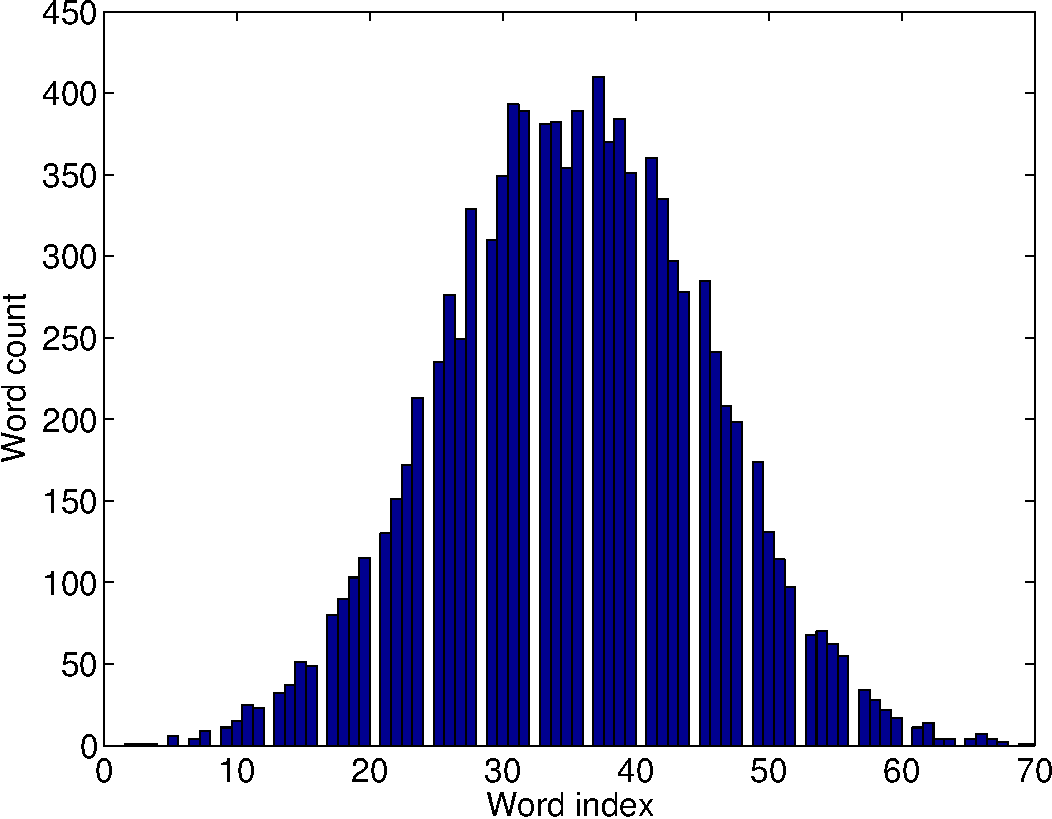
\includegraphics[width=0.8\linewidth]{histogram}
\caption{A description that makes browsing the paper easy and clearly 
describes what is in the picture. Make sure that the text in the figure 
is large enough to read and that the axes are labelled.}
\label{fig:histogram}
\end{figure}

Bla bla bla bla bla Figure~\ref{fig:histogram} bla bla bla bla bla bla 
bla bla bla bla bla bla bla bla bla bla bla bla bla bla bla bla bla 
bla bla bla bla bla bla bla bla bla bla bla bla bla bla bla bla bla 

\begin{table}
\begin{center}
\begin{tabular}{|c|c|c|}
\hline
Bla bla & Bla bla & Bla bla \\ \hline
42 & 42 & 42 \\ \hline
42 & 42 & 42 \\ \hline
\end{tabular}
\caption{A description that makes browsing the paper easy and clearly 
describes what is in the table.}
\label{tab:results}
\end{center}
\end{table}

Bla bla bla bla bla Table~\ref{tab:results} bla bla bla bla bla bla 
bla bla bla bla bla bla bla bla bla bla bla bla bla bla bla bla bla 
bla bla bla bla bla bla bla bla bla bla bla bla bla bla bla bla bla 

%%%%%%%%%%%%%%%%%%%%%%%%%%%%%%%%%%%%%%%%%%%%%%%%%%%%%%%%%%%%%
%%%%%%%%%%%%%%%%%%%%%%%%%%%%%%%%%%%%%%%%%%%%%%%%%%%%%%%%%%%%%
\section{Summary and Conclusions}
\label{sec:summary}

Bla bla bla bla bla bla bla bla bla bla bla bla bla bla bla bla bla 
bla bla bla bla bla bla bla bla bla bla bla bla bla bla bla bla bla 
bla bla bla bla bla bla bla bla bla bla bla bla bla bla bla bla bla 


%%%%%%%%%%%%%%%%%%%%%%%%%%%%%%%%%%%%%%%%%%%%%%%%%%%%%%%%%%%%%
%%%%%%%%%%%%%%%%%%%%%%%%%%%%%%%%%%%%%%%%%%%%%%%%%%%%%%%%%%%%%
\section{Contributions}
\label{sec:contributions}
We the members of project groupXX unanimously declare that 
we have all equally contributed toward the completion of this
project. (PLEASE CHANGE THIS SUITABLY WITH DETAILS, IF IT IS NOT TRUE)


%%%%%%%%%%%%%%%%%%%%%%%%%%%%%%%%%%%%%%%%%%%%%%%%%%%%%%%%%%%%%
%%%%%%%%%%%%%%%%%%%%%%%%%%%%%%%%%%%%%%%%%%%%%%%%%%%%%%%%%%%%%

\nocite{*}
\bibliographystyle{plain}
\bibliography{reflist}



\end{document}
